\chapter{系统实现}
\label{cha:implementation}

\section{开发环境与关键依赖}
\label{sec:implementation_env}

系统实现与测试在 Ubuntu 环境下完成。服务器端采用基于 Java 17 和 Spring Boot 3.4.2 的后端服务，并与 Spring Security、MySQL、Redis、MinIO、Kafka 和 Elasticsearch 等组件协同运行；客户端采用基于 Vue 3、TypeScript 与 Vite 的 Web 前端，通过浏览器访问知识库、问答和管理页面。表 \ref{tab:implementation-env} 汇总了当前实现的关键开发依赖与运行组件。

\begin{table}[H]
    \centering
    \caption{关键开发依赖与运行组件}
    \label{tab:implementation-env}
    {\small
    \begin{tabularx}{\textwidth}{L{3.1cm}Y}
        \toprule
        类别 & 组件 \\
        \midrule
        操作系统 & Ubuntu 24.04 LTS\\
        服务器端基础框架 & Java 17、Spring Boot 3.4.2 \\
        客户端基础框架 & Vue 3.5.13、TypeScript 5.8.3、Vite 6.3.5 \\
        安全依赖 & Spring Security、JWT 0.11.5 \\
        文档处理依赖 & Apache Tika 2.9.1、HanLP 1.8.6 \\
        检索依赖 & Elasticsearch Java Client 8.10.0 \\
        消息与缓存依赖 & Spring Kafka 3.2.1、Redis Starter \\
        文件存储与对象服务 & MinIO SDK 8.5.12 \\
        外部模型能力 & DeepSeek 对话接口、千问 Embedding 接口 \\
        \bottomrule
    \end{tabularx}
    }
\end{table}

\section{身份认证与组织权限实现}
\label{sec:auth_impl}

实现层首先需要解决身份与组织边界的落地问题，因为后续上传、检索、下载和问答都依赖统一的用户上下文。权限的过滤链关系如图 \ref{fig:security-filter-chain} 所示。

\begin{figure}[H]
    \centering
    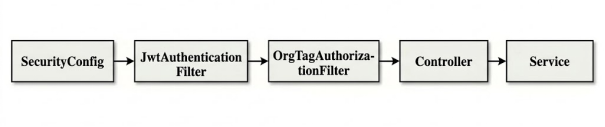
\includegraphics[width=0.85\textwidth]{image/chap04/filter.png}
    \caption{安全过滤链执行关系图}
    \label{fig:security-filter-chain}
\end{figure}

本节按照“令牌生成、注册初始化、资源过滤”三条链路展开，说明权限信息如何从登录阶段被写入系统，并持续传递到后续访问控制过程中。

\subsection{JWT 认证链路实现}

系统的认证入口位于用户登录接口。用户登录成功后，后端根据用户名查询用户实体，并在 JWT 中写入角色、用户 ID、组织标签和主组织标签等信息，为后续请求提供统一的身份上下文。

这一处理使后续模块不必重复查询完整用户对象，而能够直接基于令牌中的核心身份字段完成访问控制与上下文构建。对应的 JWT 载荷构造如下。

\begin{lstlisting}[
 numbers=left,
 basicstyle=\ttfamily,
 breaklines=true,
 keywordstyle=\color{SeaGreen4},
 caption=JWT 载荷生成,
 language=Java
]
Map<String, Object> claims = new HashMap<>();
claims.put("tokenId", tokenId);
claims.put("role", user.getRole().name());
claims.put("userId", user.getId().toString());
claims.put("orgTags", user.getOrgTags());
claims.put("primaryOrg", user.getPrimaryOrg());

String token = Jwts.builder()
        .setClaims(claims)
        .setSubject(username)
        .setExpiration(new Date(expireTime))
        .signWith(key, SignatureAlgorithm.HS256)
        .compact();
\end{lstlisting}

在请求入口处，\texttt{SecurityConfig} 负责配置认证与授权规则。系统先插入 \texttt{JwtAuthenticationFilter} 完成身份识别，再由 \texttt{OrgTagAuthorizationFilter} 执行组织标签与资源访问控制。


\subsection{私人空间与组织标签实现}

系统并未仅依赖管理员手工分配权限，而是在用户注册时自动为每个用户创建私人组织标签，并将其作为默认主组织标签。权限初始化直接放在注册环节完成，使用户首次登录后即可拥有独立的私有文档空间，而不必等待管理员额外配置。对应的初始化过程如下。

\begin{lstlisting}[
 numbers=left,
 basicstyle=\ttfamily,
 breaklines=true,
 keywordstyle=\color{SeaGreen4},
 caption=用户注册时的私人组织标签创建,
 language=Java
]
String privateTagId = PRIVATE_TAG_PREFIX + username;
createPrivateOrgTag(privateTagId, username, user);

user.setOrgTags(privateTagId);
user.setPrimaryOrg(privateTagId);
userRepository.save(user);

orgTagCacheService.cacheUserOrgTags(username, List.of(privateTagId));
orgTagCacheService.cacheUserPrimaryOrg(username, privateTagId);
\end{lstlisting}

在组织标签分配完成后，系统通过缓存服务维护用户直接标签集合与有效标签集合。这里的“有效标签”不仅包含用户显式拥有的标签，还会递归展开父级标签，用于检索与文件列表查询阶段的权限过滤。过滤的流程如图 \ref{fig:org-filter-flow} 所示。

\begin{figure}[H]
    \centering
    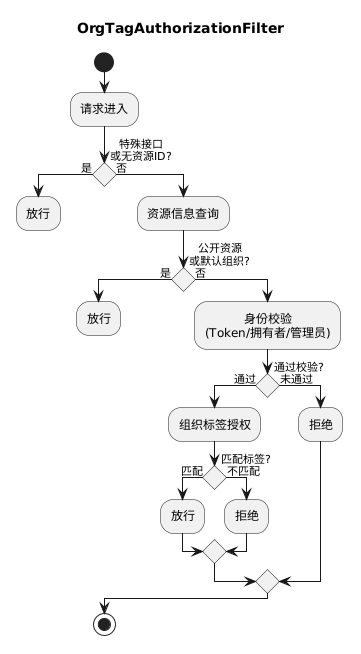
\includegraphics[width=0.45\textwidth]{image/chap04/orgfilter.png}
    \caption{组织标签授权过滤流程图}
    \label{fig:org-filter-flow}
\end{figure}

代码实现将权限控制拆分为两层：过滤器层优先完成快速身份拦截与资源访问判定，服务层再结合 \texttt{OrgTagCacheService} 的有效标签集合完成面向检索与文件列表的细粒度过滤。这种“双层校验”结构构成了当前版本的权限实现基础。

\section{文档上传与异步入库实现}
\label{sec:upload_impl}

文档入库实现横跨前端调度、对象存储和后台处理三层。本节将依次说明上传任务如何在前端形成、分片状态如何在服务端落盘、后台任务如何被投递，以及文本分块与向量索引如何最终建立。

\subsection{前端分片上传与断点续传}

前端知识库页面通过 \texttt{useKnowledgeBaseStore} 维护上传任务队列，并在 \texttt{calculateMD5} 中以 5 MB 固定粒度增量读取文件、计算 MD5。随后，前端以文件为单位串行调度分片上传请求，并根据服务端返回的 \texttt{uploadedChunks} 恢复上传位置。对应的分片调度逻辑见代码。

\begin{lstlisting}[
 numbers=left,
 basicstyle=\ttfamily,
 breaklines=true,
 keywordstyle=\color{SeaGreen4},
 caption=前端分片调度逻辑,
 language=Java
]
const totalChunks = Math.ceil(task.totalSize / chunkSize);
for (let i = 0; i < totalChunks; i += 1) {
  if (!task.uploadedChunks.includes(i)) {
    task.chunkIndex = i;
    const success = await uploadChunk(task);
    if (!success) throw new Error('分片上传失败');
  }
}
\end{lstlisting}

由于前端使用任务队列和请求取消标识维护上传状态，系统能够支持多文件排队上传，并在上传中断后继续执行未完成任务。前端因此承担了上传编排与状态恢复的第一层职责，后端则只需要关注分片接收、一致性校验与后续处理。

\subsection{服务端分片落盘与对象合并}

服务端上传接口的实现重点在于同时维护三类状态：文件记录、分片位图和对象存储。进入 \texttt{UploadService.uploadChunk} 后，系统首先确保 \texttt{file\_upload} 中存在文件记录；随后通过 Redis 位图判断分片状态，并在未上传时将分片落入 MinIO，同时补写 \texttt{chunk\_info} 表。

这种做法将“用户是否已发起上传”“某个分片是否已经存在”与“对象文件是否真正写入存储”分离处理，便于在断点续传和重复请求场景下保持一致性。相应状态维护过程如下。

\begin{lstlisting}[
 numbers=left,
 basicstyle=\ttfamily,
 breaklines=true,
 keywordstyle=\color{SeaGreen4},
 caption=分片落盘与状态维护,
 language=Java
]
if (!fileExists) {
    FileUpload fileUpload = new FileUpload();
    fileUpload.setFileMd5(fileMd5);
    fileUpload.setFileName(fileName);
    fileUpload.setTotalSize(totalSize);
    fileUpload.setStatus(0);
    fileUpload.setUserId(userId);
    fileUpload.setOrgTag(orgTag);
    fileUpload.setPublic(isPublic);
    fileUploadRepository.save(fileUpload);
}

if (!chunkUploaded) {
    String storagePath = "chunks/" + fileMd5 + "/" + chunkIndex;
    minioClient.putObject(
            PutObjectArgs.builder()
                    .bucket("uploads")
                    .object(storagePath)
                    .stream(file.getInputStream(), file.getSize(), -1)
                    .contentType(file.getContentType())
                    .build()
    );
    markChunkUploaded(fileMd5, chunkIndex, userId);
    saveChunkInfo(fileMd5, chunkIndex, chunkMd5, storagePath);
}
\end{lstlisting}

合并完成后，系统还会清理上传标记并更新文件状态，使对象一致性与业务状态推进在同一节点对齐。后续控制器正是在这一状态基础上继续发起异步入库任务。

当全部分片上传完成后，前端调用 \texttt{/api/v1/upload/merge} 触发服务端合并。合并阶段不会依赖前端的“完成标记”，而是重新检查数据库与 Redis 中的状态，以确保文件完整性。系统随后按照分片顺序构造 \texttt{ComposeSource} 列表，在 MinIO 中生成稳定对象 \texttt{merged/fileMd5}。文件合并流程如图 \ref{fig:file-merge-flow} 所示。

\begin{figure}[H]
    \centering
    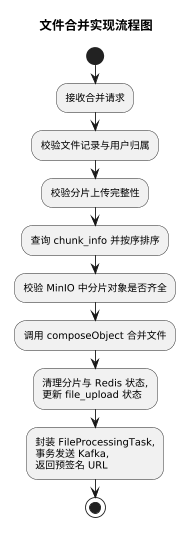
\includegraphics[height=0.42\textheight,keepaspectratio]{image/chap04/merge.png}
    \caption{文件合并实现流程图}
    \label{fig:file-merge-flow}
\end{figure}

\begin{lstlisting}[
 numbers=left,
 basicstyle=\ttfamily,
 breaklines=true,
 keywordstyle=\color{SeaGreen4},
 caption=MinIO 对象合并,
 language=Java
]
List<ComposeSource> sources = partPaths.stream()
        .map(path -> ComposeSource.builder().bucket("uploads").object(path).build())
        .collect(Collectors.toList());

minioClient.composeObject(
        ComposeObjectArgs.builder()
                .bucket("uploads")
                .object("merged/" + fileMd5)
                .sources(sources)
                .build()
);

deleteFileMark(fileMd5, userId);
fileUpload.setStatus(1);
fileUploadRepository.save(fileUpload);
\end{lstlisting}

\subsection{Kafka 异步入库与文档解析实现}

文件合并完成后，控制器将 \texttt{fileMd5}、对象访问地址、用户信息和权限信息封装为 \texttt{FileProcessingTask}，并通过事务消息发送到 Kafka。上传请求因此能够尽快返回，而解析与向量化转入后台执行。

\begin{lstlisting}[
 numbers=left,
 basicstyle=\ttfamily,
 breaklines=true,
 keywordstyle=\color{SeaGreen4},
 caption=文件处理任务投递,
 language=Java
]
FileProcessingTask task = new FileProcessingTask(
        request.fileMd5(),
        objectUrl,
        request.fileName(),
        fileUpload.getUserId(),
        fileUpload.getOrgTag(),
        fileUpload.isPublic()
);

kafkaTemplate.executeInTransaction(kt -> {
    kt.send(kafkaConfig.getFileProcessingTopic(), task);
    return true;
});
\end{lstlisting}

事务消息的作用并不只是把任务写入 Kafka，还在于将“文件已经完成合并”与“后台处理任务已经可靠投递”绑定到同一提交边界内，避免前端看到上传成功而后台处理链路尚未建立的情况。

消费者收到任务后，会先下载合并后的文件对象，再顺序调用解析服务和向量化服务。解析阶段采用 Tika 的 \texttt{AutoDetectParser} 执行流式文本提取，并在内部使用“父块缓存+子块切分”的方式避免大文件一次性读入内存；对于超长句子，则通过 HanLP 分词进一步细化切分粒度。相关逻辑如下。

\begin{lstlisting}[
 numbers=left,
 basicstyle=\ttfamily,
 breaklines=true,
 keywordstyle=\color{SeaGreen4},
 caption=流式解析与语义切分,
 language=Java
]
try (BufferedInputStream bufferedStream =
        new BufferedInputStream(fileStream, bufferSize)) {
    StreamingContentHandler handler =
            new StreamingContentHandler(fileMd5, userId, orgTag, isPublic);
    AutoDetectParser parser = new AutoDetectParser();
    parser.parse(bufferedStream, handler, metadata, context);
}

@Override
public void characters(char[] ch, int start, int length) {
    buffer.append(ch, start, length);
    if (buffer.length() >= parentChunkSize) {
        processParentChunk();
    }
}
\end{lstlisting}

\subsection{向量化与索引写入实现}

向量化阶段由 \texttt{VectorizationService} 驱动。系统先从 \texttt{document\_vectors} 中读取同一文件的全部文本分块，再通过 \texttt{EmbeddingClient} 批量调用嵌入接口生成 2048 维向量，最终组装为 \texttt{EsDocument} 批量写入 \texttt{knowledge\_base} 索引。其关键代码如下。

\begin{lstlisting}[
 numbers=left,
 basicstyle=\ttfamily,
 breaklines=true,
 keywordstyle=\color{SeaGreen4},
 caption=向量生成与索引写入,
 language=Java
]
List<TextChunk> chunks = fetchTextChunks(fileMd5);
List<String> texts = chunks.stream()
        .map(TextChunk::getContent)
        .toList();
List<float[]> vectors = embeddingClient.embed(texts);

List<EsDocument> esDocuments = IntStream.range(0, chunks.size())
        .mapToObj(i -> new EsDocument(
                UUID.randomUUID().toString(),
                fileMd5,
                chunks.get(i).getChunkId(),
                chunks.get(i).getContent(),
                vectors.get(i),
                "deepseek-embed",
                userId,
                orgTag,
                isPublic
        ))
        .toList();

elasticsearchService.bulkIndex(esDocuments);
\end{lstlisting}

这种写法将分块内容、权限元数据与向量结果一次性拼装为索引文档，减少了写入阶段的中间转换。检索阶段也能够直接依据 \texttt{userId}、\texttt{orgTag} 和公开属性执行过滤。

\section{混合检索与流式问答实现}
\label{sec:chat_impl}

检索问答实现的关键不在于单个接口是否可调用，而在于检索、会话状态和流式输出是否共享同一上下文。只有这三部分保持连续，系统才能把权限受限的候选知识稳定转化为可消费的回答结果。因此，本节依次说明候选召回、提示词组织与 WebSocket 事件流的具体实现。

\subsection{混合检索实现}

系统的混合检索由 \texttt{HybridSearchService} 实现，其实现重点不在于机械叠加多种检索手段，而在于把召回、权限与排序压缩到一次 Elasticsearch 查询中。这样可以尽量减少候选结果在应用层的多次搬运与重复过滤。

服务首先根据用户身份获取有效组织标签集合，再调用嵌入接口为当前问题生成查询向量。如果向量生成失败，系统会直接降级到纯文本检索路径；若向量生成成功，则在同一次 Elasticsearch 请求中完成 kNN 召回、权限过滤与 \texttt{rescore} 二阶段重排序。相应查询构造如下。

\begin{lstlisting}[
 numbers=left,
 basicstyle=\ttfamily,
 breaklines=true,
 keywordstyle=\color{SeaGreen4},
 caption=混合检索与权限过滤,
 language=Java
]
int recallK = topK * 30;

s.knn(kn -> kn
        .field("vector")
        .queryVector(queryVector)
        .k(recallK)
        .numCandidates(recallK)
);

s.query(q -> q.bool(b -> b
        .must(m -> m.match(ma -> ma.field("textContent").query(query)))
        .filter(f -> f.bool(bf -> bf
                .should(s1 -> s1.term(t -> t.field("userId").value(userDbId)))
                .should(s2 -> s2.term(t -> t.field("public").value(true)))
                .should(s3 -> /* org tag filter */ s3)
        ))
));

s.rescore(r -> r
        .windowSize(recallK)
        .query(rq -> rq
                .queryWeight(0.2d)
                .rescoreQueryWeight(1.0d)
                .query(rqq -> rqq.match(m -> m
                        .field("textContent")
                        .query(query)
                        .operator(Operator.And)
                ))
        )
);
\end{lstlisting}

该实现的特点有两点：一是权限过滤在候选召回阶段就已经参与执行，而不是在结果返回后再二次裁剪；二是文本重排序直接利用 Elasticsearch 提供的 \texttt{rescore} 机制完成，不需要在应用层手工维护额外排序器。

\subsection{会话状态与提示词编排实现}

在问答链路中，\texttt{ChatHandler} 负责管理对话状态。系统首先在 Redis 中读取或创建用户当前会话标识，再读取该会话对应的历史消息列表；随后使用检索结果构造来源上下文，并把它们与系统规则一起送入 \texttt{DeepSeekClient}。

为了控制上下文规模，系统会将历史消息数量限制在最近 20 条以内，避免会话无限增长后挤占有效证据片段。其关键逻辑如下。

\begin{lstlisting}[
 numbers=left,
 basicstyle=\ttfamily,
 breaklines=true,
 keywordstyle=\color{SeaGreen4},
 caption=会话历史读取与上下文构建,
 language=Java
]
String conversationId = getOrCreateConversationId(userId);
List<Map<String, String>> history = getConversationHistory(conversationId);
List<SearchResult> searchResults =
        searchService.searchWithPermission(userMessage, userId, 5);
String context = buildContext(searchResults, session.getId());
\end{lstlisting}

由于会话标识、历史消息和检索结果都在服务端显式组织，前端不需要自行拼接模型输入，这使对话状态能够与权限检索结果保持一致，也降低了客户端状态漂移的风险。

在 \texttt{DeepSeekClient} 中，系统将检索结果包装在统一的引用定界符之间，并将“仅依据参考资料作答、无结果时明确说明”等规则写入系统指令。该设计保证了模型回答尽可能受检索证据约束，对应装配过程如下。

\begin{lstlisting}[
 numbers=left,
 basicstyle=\ttfamily,
 breaklines=true,
 keywordstyle=\color{SeaGreen4},
 caption=提示词装配逻辑,
 language=Java
]
StringBuilder sysBuilder = new StringBuilder();
sysBuilder.append(promptCfg.getRules()).append("\n\n");
sysBuilder.append(refStart).append("\n");

if (context != null && !context.isEmpty()) {
    sysBuilder.append(context);
} else {
    sysBuilder.append(promptCfg.getNoResultText()).append("\n");
}

sysBuilder.append(refEnd);
messages.add(Map.of("role", "system", "content", sysBuilder.toString()));
\end{lstlisting}

\subsection{WebSocket 流式交互实现}

前端聊天模块通过 \texttt{@vueuse/core} 提供的 \texttt{useWebSocket} 建立长连接，并在连接建立后接收后端返回的 \texttt{sessionId}。后端在 \texttt{ChatWebSocketHandler} 中解析 JWT、识别用户，再将普通文本消息转交给 \texttt{ChatHandler} 处理。

因此，聊天状态流并不是单向文本回传，而是包含连接建立、消息发送、增量内容推送、完成通知和引用映射清理等一组连续事件。前端会话状态维护逻辑如下。

\begin{lstlisting}[
 numbers=left,
 basicstyle=\ttfamily,
 breaklines=true,
 keywordstyle=\color{SeaGreen4},
 caption=前端 WebSocket 会话状态维护,
 language=Java
]
const { data: wsData, send: wsSend } =
  useWebSocket(`/proxy-ws/chat/${store.token}`, { autoReconnect: true });

watch(wsData, (val) => {
  if (!val) return;
  const data = JSON.parse(val);
  if (data.type === 'connection' && data.sessionId) {
    sessionId.value = data.sessionId;
  }
});
\end{lstlisting}

在流式返回过程中，后端将模型增量内容包装为 \texttt{\{"chunk": "..."\}} 的 JSON 消息逐段发送给前端，并在回答结束时再发送完成通知。与此同时，系统维护“引用编号到文件 MD5”的映射关系，为后续来源定位和下载操作提供依据，至此形成从权限检索、上下文组织到流式问答输出的完整闭环实现。
